\documentclass[11pt]{article}

\usepackage[spanish]{babel}
\usepackage{translations}
\usepackage[titles]{tocloft}
\usepackage{multicol}
\usepackage{graphicx}
\usepackage{amsmath}
\usepackage{hyperref}
\usepackage{amsmath}
\usepackage{amssymb}
\usepackage{listings}
\usepackage{courier}
\usepackage[margin=1in]{geometry}
\usepackage{changepage}
\usepackage{titlesec}
\usepackage{wrapfig}
\usepackage[version=4]{mhchem}
\usepackage{multirow}
\usepackage{siunitx}
\usepackage{ragged2e}
\usepackage{adjustbox}
\usepackage[font=small,labelfont=bf]{caption}
\usepackage[table,xcdraw]{xcolor}
\usepackage{afterpage}
\usepackage{xfrac}
\usepackage{animate}
\usepackage{subcaption}
\usepackage{tcolorbox}
\usepackage{nicefrac}

\setlength{\parindent}{1cm}

\definecolor{mytheoremfr}{HTML}{7B0000}
\definecolor{mytheorembg}{HTML}{f5e4e1}

\tcbuselibrary{theorems,skins,hooks}
\newtcbtheorem[number format=\alph]{Theorem}{Pregunta}
{%
	enhanced,
	colback = mytheorembg,
	frame hidden,
	boxrule = 0sp,
	borderline west = {2pt}{0pt}{mytheoremfr},
	sharp corners,
	detach title,
	before upper = \tcbtitle,
	coltitle = mytheoremfr,
	fonttitle = \bfseries\sffamily,
	description font = \mdseries,
	separator sign none,
	segmentation style={solid, mytheoremfr},
}
{th}

\usetikzlibrary{arrows,calc,shadows.blur}
\tcbuselibrary{skins}
\newtcolorbox{note}[1][]{%
	enhanced jigsaw,
	colback=gray!10!white,%
	colframe=gray!80!black,
	size=small,
	boxrule=1pt,
	title=\textbf{Cuestión:},
	halign title=flush center,
	coltitle=black,
	drop shadow=black!50!white,
	attach boxed title to top left={xshift=1cm,yshift=-\tcboxedtitleheight/2,yshifttext=-\tcboxedtitleheight/2},
	minipage boxed title=2.5cm,
	boxed title style={%
			colback=white,
			size=fbox,
			boxrule=1pt,
			boxsep=2pt,
			underlay={%
					\coordinate (dotA) at ($(interior.west) + (-0.5pt,0)$);
					\coordinate (dotB) at ($(interior.east) + (0.5pt,0)$);
					\begin{scope}[gray!80!black]
						\fill (dotA) circle (2pt);
						\fill (dotB) circle (2pt);
					\end{scope}
				},
		},
	#1,
}

\newcommand{\preguntaAlaMadreDeRocio}[1]{\begin{Theorem}{#1}{}\end{Theorem}}
\newcommand{\laputa}[1]{\begin{note}{#1}{}\end{note}}

\renewcommand{\labelenumi}{\alph{enumi}.}
   
\newcommand{\titulo}{Estudio del movimiento de un\\ cuerpo en un campo central\\
de fuerza\\\ \\(Práctica 2)}
\newcommand{\nombreestudiante}{Víctor Mira Ramírez}
\newcommand{\nombredirector}{Luis Antón Ruiz}
\newcommand{\fecha}{\date{Diciembre 2023}}

\pagebreak

\renewcommand{\listtablename}{Índice de tablas} 
\renewcommand{\tablename}{Tabla} 
\renewcommand\cftsecdotsep{\cftdotsep}

\setlength{\cftbeforesecskip}{0.5ex}
\renewcommand{\cftsecfont}{%
  \fontsize{11}{13}\usefont{OT1}{phv}{bc}{n}\selectfont
}
\makeatletter
\renewcommand{\@pnumwidth}{1.75em}
\renewcommand{\@tocrmarg}{2.75em}
\makeatother

\begin{document}
    \begin{titlepage}
    	\centering
    	
\includegraphics[width=65mm]{fotos/logoUA.png}\par
    	\vspace{1cm}
    	{\huge\bfseries \vspace{15mm} \titulo \par}
    	\vfill
    	{\large 
    	\vfill
    	Estudiante:\par\vspace{2mm}
    	\nombreestudiante\par
    	\vfill
    	Profesor:\par\vspace{2mm}
        \nombredirector
        \vfill
        Universidad de Alicante\par
        Facultad de Ciencias: Departamento de Física Aplicada\par
        Mecánica Newtoniana y Relatividad\par
    	\fecha\par}
    \end{titlepage}
    
    \clearpage

    \begin{abstract}\label{sec:abstract}
        Este informe examina el comportamiento de un cuerpo sometido a un campo central de fuerzas. Se discutirá la interacción gravitatoria terrestre sobre un satélite que orbita al planeta Tierra.
    \end{abstract}\vspace{0.3cm}  
    
    \tableofcontents
    \clearpage
    \section{Cuestiones propuestas}
        \laputa{Considera a La Tierra como fuente de interacción gravitatoria (busca su masa y su radio). Busca también el rango de masa que suelen tener los satélites artificiales.\\
        
        ¿El código mantiene una órbita circular? ¿El valor del radio es constante? ¿El periodo es correcto?         
        \[T=2\pi\sqrt{\dfrac{R^3}{G\mu}}\]}

            \noindent Datos literatura:\\
            
            \vspace{-0.1cm}$\left\{\begin{aligned}
                &\text{Masa terrestre: }M=5.972\cdot10^{24}\ kg\\
                &\text{Radio terrestre: }R=6.371\cdot10^6\ m\\
                &\text{Masa satélite artificial: }m=750\ kg
            \end{aligned}\right.$\\

            \noindent La órbita obtenida no es circular ya que el valor del radio no es constante. El valor del periodo coincide con el visto en las clases de teoría.
        
        \laputa{Sitúa el satélite de forma que haga una órbita de perigeo aproximadamente $300$ km sobre la superficie terrestre. Dibuja el potencial efectivo en ese caso e indica en el gráfico la distancia mínima y máxima al centro de la tierra. Obtén $r(t)$ y $v(t)$. ¿Los valores del apogeo son correctos? ¿Y el periodo? 
        \[T=2\pi\sqrt{\dfrac{a^3}{G\mu}}\]
        donde $a$ es el semieje mayor de la elipse
        \[a=\dfrac{r_\text{apogeo}+r_\text{perigeo}}{2}\]}

            \begin{wrapfigure}[12]{l}{0.48\textwidth}
                \vspace{-0.42cm}
                \centering
                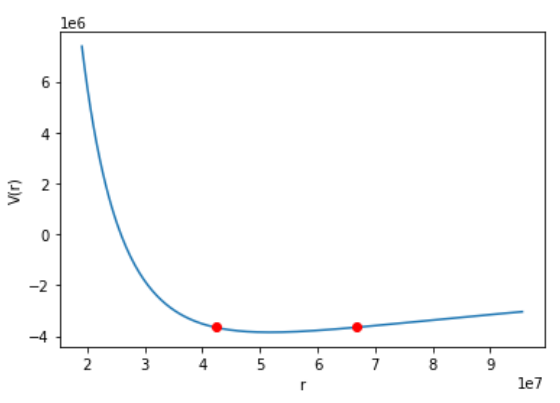
\includegraphics[width=0.46\textwidth]{fotos/graficas/1.png}
            \end{wrapfigure}

            \hspace{0cm}\\\noindent Vamos a representar el potencial efectivo en una gráfica. Donde la energía mecánica total y el potencial efectivo se cortan tenemos el perigeo y el apogeo de la órbita del satélite alrededor a La Tierra. La distancia máxima la tenemos en el perigeo y la mínima en el apogeo.            
            \[\left\{\begin{aligned}
                r_\text{apogeo}= 6.667\cdot 10^{7}\ m\\
                r_\text{perigeo}=4.238\cdot 10^{7}\ m
            \end{aligned}\right.\]

            \hspace{0cm}\\\hspace{0cm}\\\noindent Vemos que la órbita es elíptica pues tiene perigeo y apogeo. Para lograr obtener las ecuaciones del movimiento hemos de hacer uso de la librería \textit{odeint} de \textit{Python}. Sabemos por las clases de teoría que las órbitas en potenciales pequeños corresponden a órbitas elípticas, que es el caso que observamos. Vemos también que el mínimo de energía no coincide en un punto, lo cual indicaría que nuestra órbita es circular.

        \clearpage
        \laputa{Varía las condiciones iniciales para representar los tres tipos de trayectoria que pueden darse en este problema. Siempre dibuja el potencial efectivo, situando la energía total en el gráfico. Haz una animación de cada trayectoria, de tal manera que se vea la trayectoria del satélite a medida que avanza el tiempo.}

            \vspace{-0.2cm}
            \subsubsection*{Órbita circular/elíptica}
            \vspace{-0.2cm}
            $E_\text{total}=E_\text{min}\Longrightarrow v=\sqrt{\dfrac{GM}{fR}}$
            con $1< f < 2$ siendo $f=1$ en el caso circular.

            \begin{figure}[h]
                \centering
                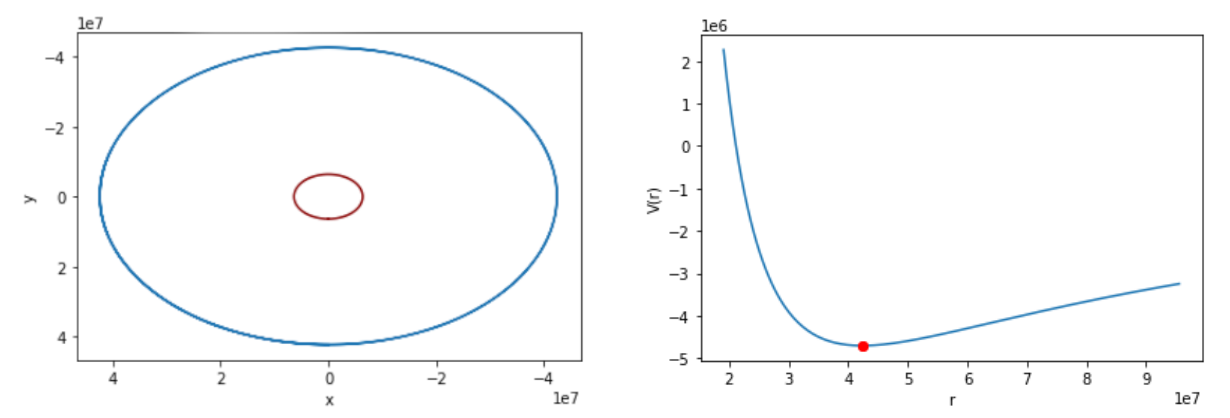
\includegraphics[width=0.8\textwidth]{fotos/graficas/circular.png}
            \end{figure}
            
            \vspace{-0.9cm}
            \subsubsection*{Órbita parabólica}
            \vspace{-0.2cm}
            $0>E_\text{total}>E_\text{min}\Longrightarrow v=\sqrt{\dfrac{GM}{2R}}$

            \begin{figure}[h]
                \centering
                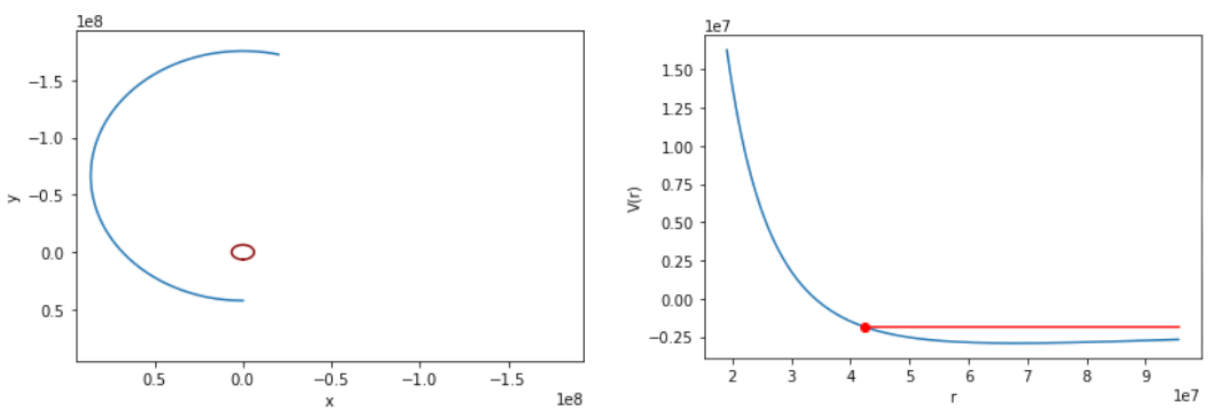
\includegraphics[width=0.8\textwidth]{fotos/graficas/parabolica.png}
            \end{figure}

            \vspace{-0.9cm}
            \subsubsection*{Órbita hiperbólica}
            \vspace{-0.2cm}
            $E_\text{total}>0\Longrightarrow v=\sqrt{\dfrac{GM}{fR}}$
            con $f>2$

            \begin{figure}[h]
                \centering
                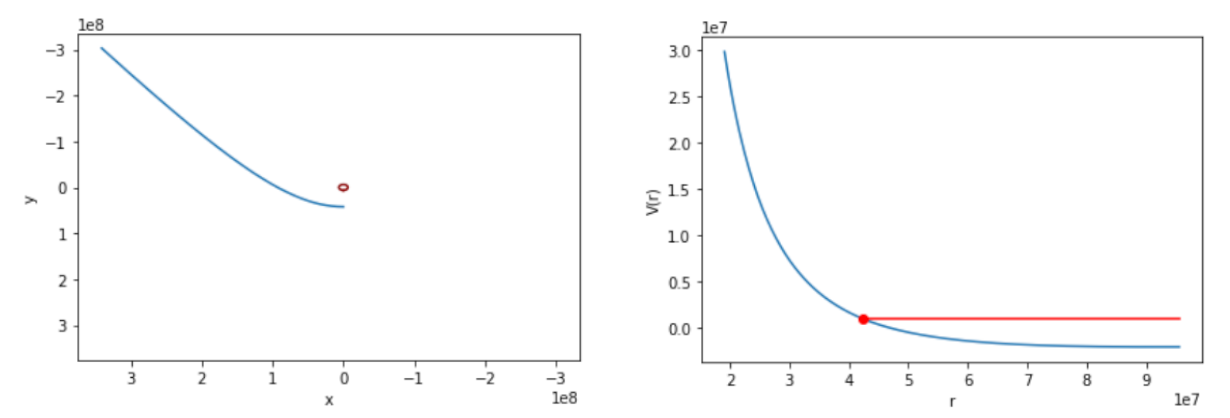
\includegraphics[width=0.8\textwidth]{fotos/graficas/hiperbolica.png}
            \end{figure}

        \clearpage
        \laputa{En el caso de las órbitas acotadas, resuelve las ecuaciones considerando el potencial que obtuviste en el problema 3 del boletín 1 y haz una animación de lo que sucede en este caso.
        \[V(r)=\dfrac{A}{r^5}\]
        Donde para que se describa una circunferencia de radio $R$ que acabe en la fuente de potencial se ha de cumplir que $A=\dfrac{8(LR)^2}{m^2}$. Donde $L$ es el momento angular del cuerpo y $m$ la masa del cuerpo.}

            \begin{wrapfigure}[12]{l}{0.52\textwidth}
                \vspace{-0.3cm}
                \centering
                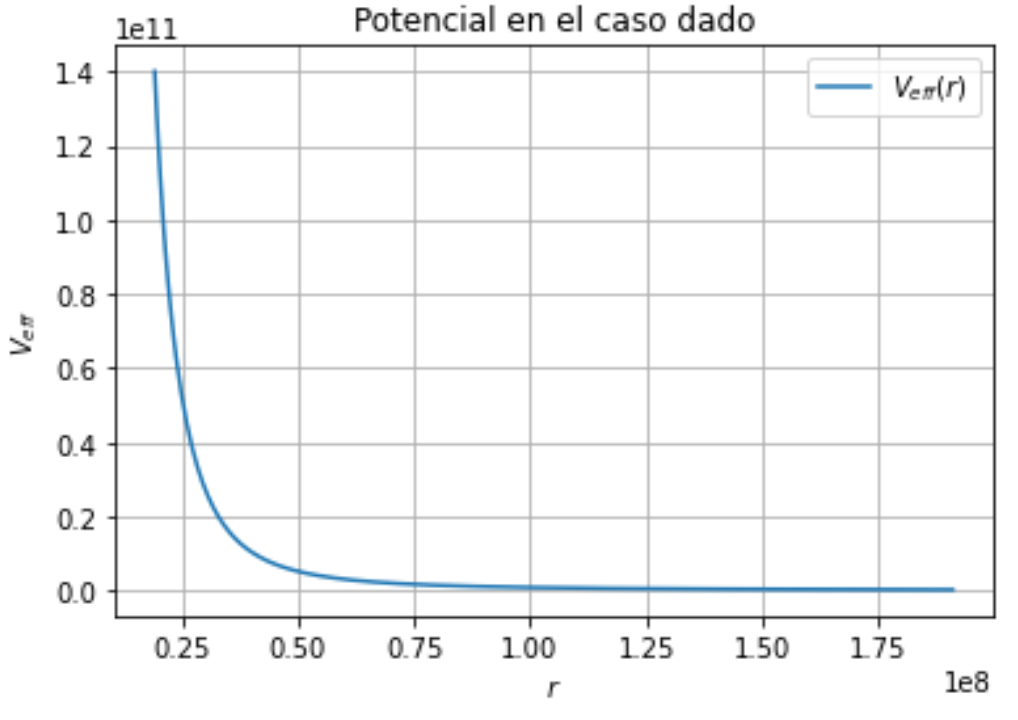
\includegraphics[width=0.51\textwidth]{fotos/graficas/5.png}
            \end{wrapfigure}
            
            \hspace{0cm}\\\hspace{0cm}\\\hspace{0cm}\\\noindent En el ejercicio nombrado se nos pide demostrar que si una partícula se encuentra sometida a una fuerza central atractiva hacia un punto de su órbita la fuerza es inversamente proporcional a la distancia al centro de fuerzas con la quinta potencia.\\\hspace{0cm}\\\hspace{0cm}\\\hspace{0cm}\\
    
            \noindent Basta integrar la expresión de $F=-\dfrac{8(LR)^2}{mr^5}\hat{r}$ para obtener la expresión del potencial $U(r)$, al cual sumándole $\dfrac{L^2}{2mr^2}$ obtenemos el potencial efectivo que buscamos y vemos en la gráfica.

            \[V_\text{eff}(r)=\int F\ dr+\dfrac{L^2}{2mr^2}\]

        \hspace{0cm}\\
        \laputa{Repite el análisis para el potencial de un muelle. ¿Cuántos tipos de trayectoria hay en este caso? ¿Son cerradas?}

            \noindent Como nos hallamos ahora en el caso en el que tenemos energías muy bajas, el potencial efectivo puede ser representado con un desarrollo limitado de segundo orden que corresponderá con un movimiento oscilatorio:
            \[V_\text{eff}(r)=V_\text{eff}(r_\text{min})+\dfrac{1}{2}k(r-r_\text{min})^2\]
    
            \noindent Si tomamos como constante del muelle $k=1$ y la masa $m=1$ obtenemos las gráficas para el muelle. Como la energía es negativa pero es mayor que la energía mínima sólo tendremos un tipo de órbita: elíptica (órbita cerrada).

        \clearpage
        \laputa{Por último, agrega al potencial del muelle un término proporcional a $r^3$, es decir, un término de fuerza proporcional a $r^2$. Haz una animación de la trayectoria en este caso y explica lo que sucede.}

            \begin{wrapfigure}[11]{l}{0.5\textwidth}
                \vspace{-0.4cm}
                \centering
                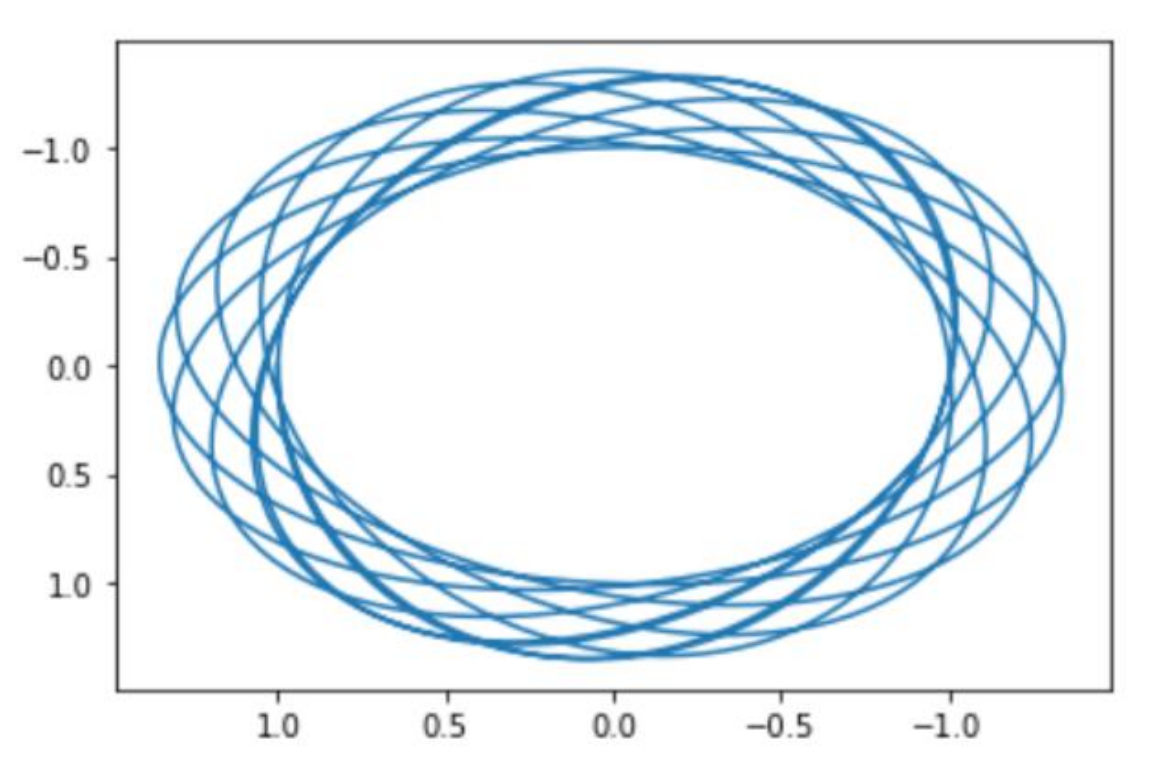
\includegraphics[width=0.5\textwidth]{fotos/graficas/7.png}
            \end{wrapfigure}
            
            \hspace{0cm}\\\noindent Si añadimos un término proporcional a $r^3$:
            \[E_\text{mec}=\dfrac12 mv^2+\dfrac13 kr^3\]

            \noindent Observamos como la órbita es elíptica como en el caso anterior y además en un rango similar de energías, solo que esta vez la trayectoria elíptica rota con el tiempo, dando lugar con el tiempo a una órbita definida entre dos radios, uno máximo y uno mínimo.
    \section{Anexos}
        \subsubsection*{Código de LaTeX que genera este documento:}
            \href{https://www.overleaf.com/read/trvqgmfvrzfv#d29911}{MECN-Practica2:central.tex}

\end{document} 